% ==================================================================================================================
\section{Z�rich}
\label{sec:zhscenario}
\hfill \textbf{Author:} Andreas Horni

The Z�rich scenario is probably the most used scenario in MATSim community. Its base is the Switzerland scenario described above. The Z�rich scenario, however, is the more detailed scenario; it is enhanced by data only available for the smaller region, e.g., traffic light data or freight demand data is only included for Z�rich city and canton respectively. It is under continuous development, calibration and validation. It has been applied in numerous projects and and serves as a real-world example for research.   

\citet{HorniEtAl_TechRep_IVT_2011_a} provides a technical overview of the first branch of the scenario. \citet[][]{BalmerEtAl_ResRep_bdktzrh_2009} describes its generation in the context of the project ``Westumfahrung. 

The Zurich base scenario is a cut-out from the Switzerland scenario described above. The study area is delineated by a circle with a 30~km radius around Bellevue, a central and prominent location in Z�rich. This delineation leads to two version, namely the \emph{Z�rich diluted scenario} and the \emph{Z�rich cut scenario}. For the first one, all agents crossing the study area in the simulated day are considered (Figure \ref{fig:zurichScenario}), which results in almost 2 million agents. For the second, only the agents staying within this area are modeled. The \emph{Z�rich cut scenario} has been used in an experimental manner only in \citet[][]{Hackney_PhDThesis_2009}. It is thus recommended to use the \emph{Zurich diluted scenario} for production runs.

Demand is directly taken from the Swiss model. Additionally, freight traffic has been added to the Z�rich scenario as follows. Canton Zurich raw data for freight traffic is taken from the \emph{KVM} (Kantonales Verkehrsmodell) provided by \citet{AMV_Webpage_2011} and documented in \citet[][]{GottardiBuergler_SV_1999}. Matrices given at zonal level are disaggregated to single MATSim plans \citep[][]{ShahM_TechRep_IVT_2010}. Matrices for small delivery trucks and heavy trucks are combined into one activity called \emph{freight}. An additional 180'000 agents are generated for the Z�rich region.

For the diluted Z�rich scenario all Swiss facilities as described above are used as activity locations. For the diluted scenario, the networks are not thinned out. For the public transport simulation a network from the \emph{KVM} (Kantonales Verkehrsmodell Z�rich) as provided by \citet[][]{AMV_Webpage_2011} is used. 

The scenario simulates car and recently also public transport. Public transport schedules are derived from the KVM ZH. The modes walk and bike are ``teleported''. 

Calibration is mainly done for modal split and distance distributions. Utility function values are set accordingly.

For validation, count data on city level, cantonal level and national level \citep[][]{ASTRA_Webpage_2006} are available from various sources resulting in 123 links measured for the inner city of Z�rich delineated by a 12~km radius around Bellevue. The reduced radius of count analysis is applied to reduce boundary effects given by the reduction of demand considered outside the 30~km radius study area. An average working day (Monday to Thursday, excluding public holidays) is used for comparisons in current scenarios.

Traffic signal data are available for the city of Z�rich \citep[][]{STAPOZH-DAV_unpub_gtZH_2008}. They have been integrated for the project Westumfahrung.

\createfigure%
{The Diluted Z�rich Scenario}%
{The Diluted Z�rich Scenario}%
{\label{fig:zurichScenario}}%
{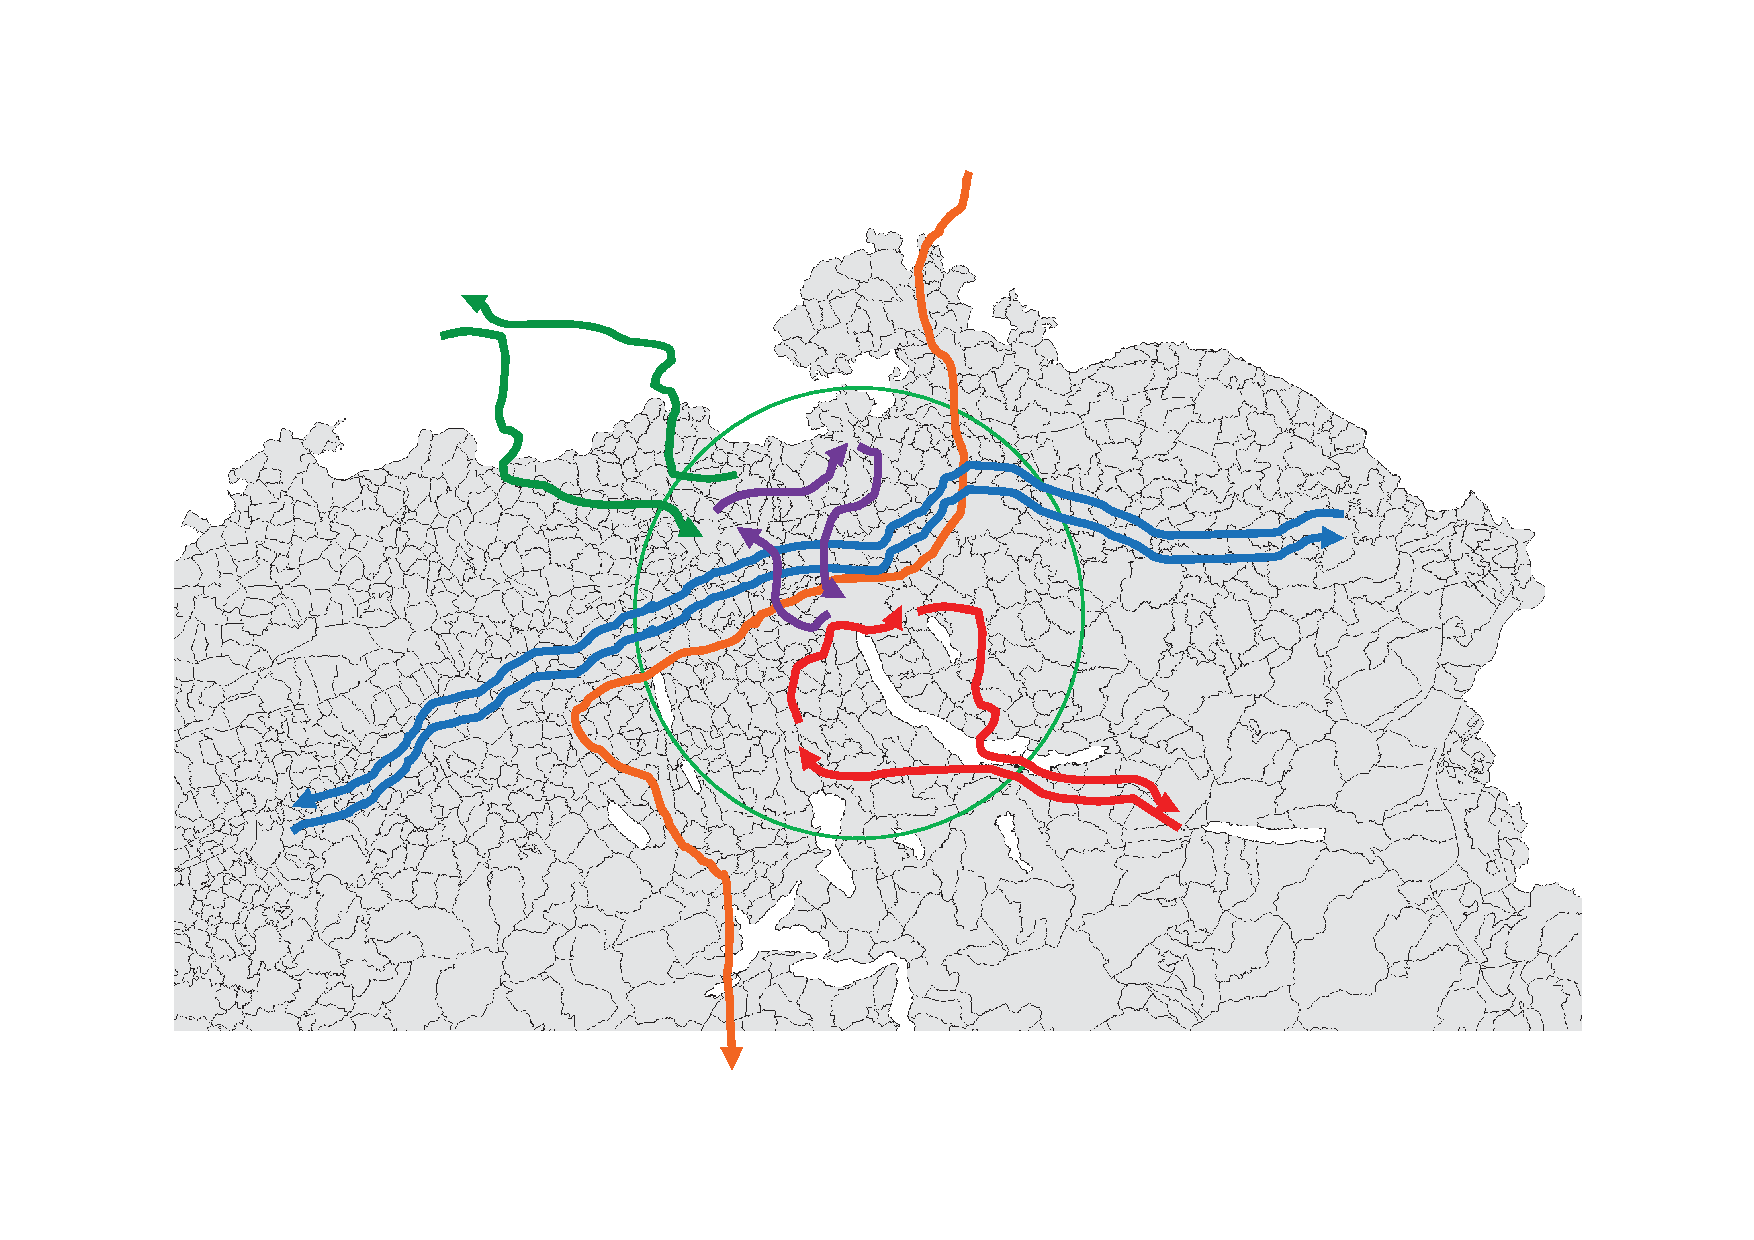
\includegraphics[width=0.99\textwidth, angle=0]{using/figures/zh.pdf}}%
{}

% ==================================================================================================================
